\section{Project Management}

\subsection{Professional, Legal, Ethical, and Social Issues}

\subsubsection{Professional Issues} \mbox{} \\

All software development carried out during this project will adhere to the British Computing Society (BCS) code of conduct. Furthermore, every evaluation in this project will be conducted rationally and without bias, using objective metrics and the critical analysis of results.

\subsubsection{Legal Issues} \mbox{} \\

To carry out the project, third-party software is required. To ensure legal compliance, any third-party software will be used in accordance with its respective licensing terms.

\subsubsection{Ethical Issues} \mbox{} \\

Since this project guarantees the soundness of the proof checker, that is, if the checker validates a DNN verification query, then the result is guaranteed to hold, the implementation must be free of any bugs that could compromise this guarantee. Therefore, the project will take advantage of Rocq's type checker as the primary correctness mechanism, ensuring that all definitions and proofs are verified before being considered complete. Additionally, the implementation will be tested thoroughly against benchmarks to confirm that the checker behaves as expected in practice.

\subsubsection{Social Issues} \mbox{} \\

The social implications of this project centre on improving the accessibility of certified verification tools within the DNN verification landscape. By translating the proof checker into Rocq, a more widely adopted proof assistant, the project aims to broaden the community engaged in certified DNN verification. Ultimately, the project does not pose any direct social issues.

\subsection{Project Planning}

The Gantt chart shown in \autoref{fig:gantt_chart} illustrates the project tasks and their respective projected durations.

\subsubsection{Gantt Chart} \mbox{} \\

\begin{figure}[h]
    \centering
    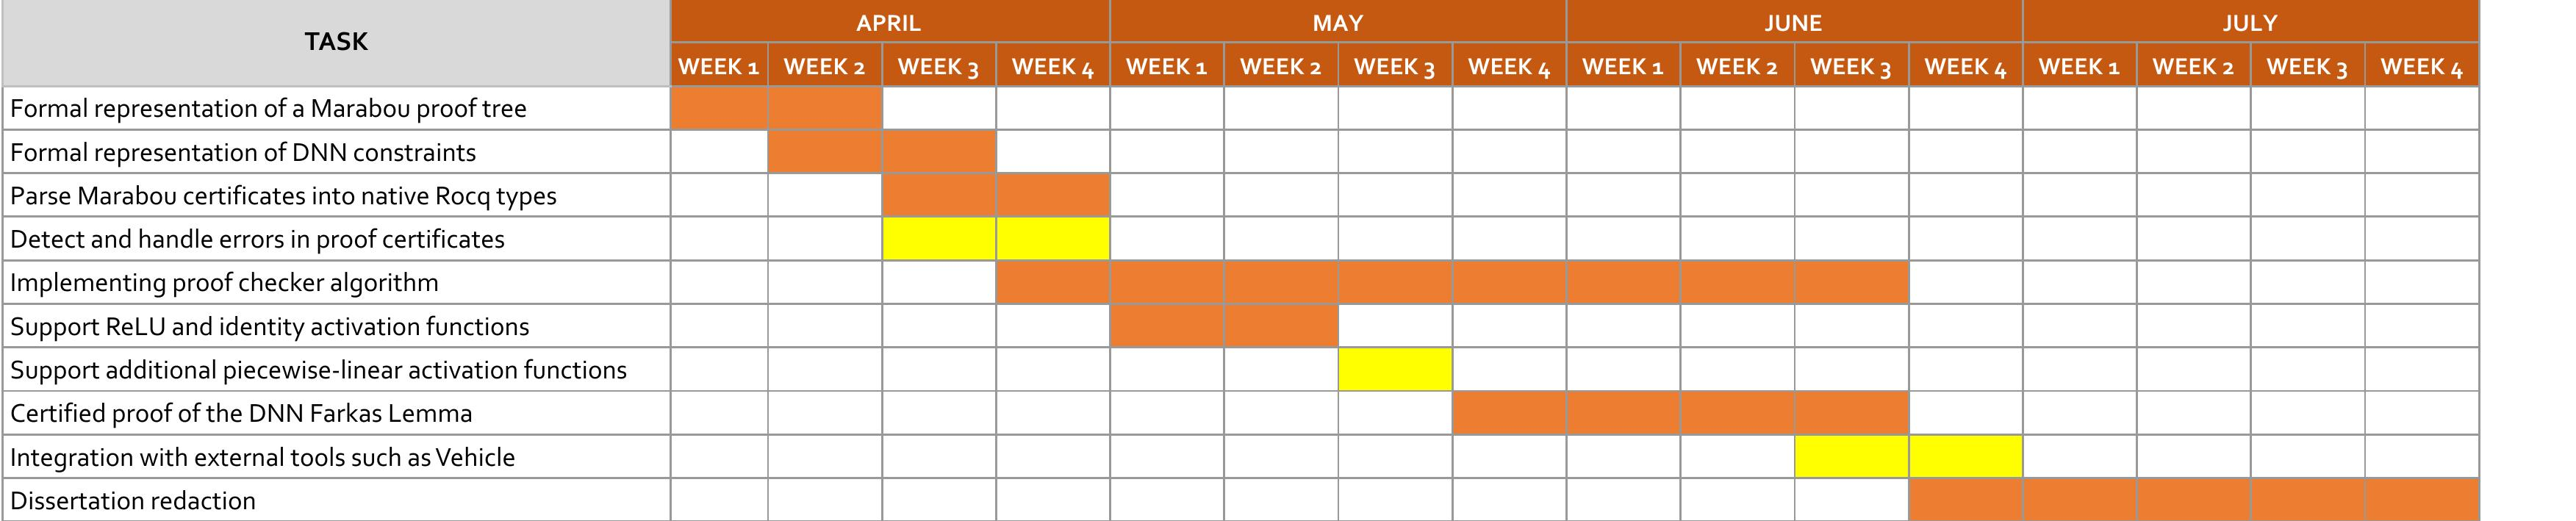
\includegraphics[width=\textwidth]{images/gantt_chart.jpg}
    \caption{Project Gantt Chart}
\end{figure}
\label{fig:gantt_chart}

\subsubsection{Risk Analysis} \mbox{} \\

In \autoref{tab:risk-analysis}, a list of possible adverse consequences, their impact, likelihood and mitigation plan is shown.

\begin{table}[h]
\centering
\begin{tabularx}{\textwidth}{X c c}
\toprule
\textbf{Risk} & \textbf{Impact} & \textbf{Likelihood} \\
\midrule
Type system incompatibilities between Imandra and Rocq & Medium & Medium \\
Untranslatable proof strategy from Imandra & High & Medium \\
Missing mathematical foundations in Rocq standard library & High & Medium \\
Rocq termination checker rejects recursive functions & Medium & Medium \\
Marabou certificate format changes between versions & Medium & Low \\
Scope too large to complete within project timeline & High & Medium \\
Incompatible changes in the Imandra proof checker & Low & Low \\
\bottomrule
\end{tabularx}
\caption{Risk Analysis. For each risk, a mitigation plan is outlined below.}
\label{tab:risk-analysis}
\end{table}

\paragraph*{Type system incompatibilities between Imandra and Rocq.} Fundamental differences between the two types of theorem proving may preclude the symmetric translation of certain definitions. The mitigation plan is to thoroughly analyse the Imandra implementation before beginning the translation, identifying any incompatibilities early and adjusting the data constructs accordingly.

\paragraph*{Missing mathematical foundations in Rocq standard library.} Rocq's standard library may not provide all the necessary tools to carry out the proof. The mitigation plan is to identify alternative libraries early in the project, such as MathComp and make use of them.

\paragraph*{Untranslatable proof strategy from Imandra.} Imandra relies heavily on automated reasoning, meaning that certain proof steps may have no direct equivalent in Rocq's interactive tactic system. In such cases, the mitigation plan is to identify an alternative proof strategy and prove it manually within the Rocq proof system.

\paragraph*{Marabou certificate format changes between versions.} The format of proof certificates produced by Marabou may vary across versions, which could compromise the compatibility of the generated certificates with those expected by the proof checker. Since Marabou is an open-source, Git-hosted project, the mitigation strategy is to pin the implementation to a specific version of Marabou using Git's versioning features. \label{risk:marabou_version}

\paragraph*{Scope too large to complete within the project timeline.} The full translation of the proof checker may require more time than was initially considered. The mitigation plan is to prioritise the reconstruction of the validity algorithm and treat the formal soundness proof as a complementary goal.

\paragraph*{Incompatible changes in the Imandra proof checker.} Although the Imandra proof checker has not received any recent contributions, it may undergo any development during the course of this project. Such changes could result in incompatibilities with the ongoing implementation. Similarly to \autoref{risk:marabou_version}, given that the Imandra proof checker is an open-source, Git-hosted project, the proposed mitigation is to pin the implementation to a specific version.
